% ==========================================================================
% MergeSpec method subsections 2 & 3:
%   "Expert Relation Map" + "Relation-Guided Cluster-and-Merge"
% Insert AFTER \subsection{Why Expert Merging Preserves Draft Coverage},
% BEFORE the (upcoming) merge-system-optimization subsection
% (to be written next session).
%
% Notation is inherited from the draft: layer $\ell$, $n$ experts, top-$k$
% set $\mathcal{T}_{\ell,t}$, expert $E_{\ell,i}$, hidden state $h_{\ell,t}$,
% budget $K$, groups $\mathcal{C}_{\ell,j}$, merged expert
% $\widehat{E}_{\ell,j}$ with weights $\alpha_{\ell,j,i}$ (Eq. 5), expert
% weights $\mathbf{W}_{\ell,i}$ / merged $\widehat{\mathbf{W}}_{\ell,j}$
% (Proposition 2 proof, Eq. 9), cycle $s$, speculation length $\gamma$.
% NEW symbols introduced here:
%   $\mathbf{A}_\ell$ (activation-similarity map),
%   $\mathbf{C}_\ell$ (co-occurrence map),
%   $\mathbf{R}_\ell$ (blended relation map),
%   $\lambda$ (blend coefficient — NOT $\alpha$, which Eq. 5 already uses),
%   $\mathcal{P}_\ell^{ij}$ (prefill co-routed tokens),
%   $\mathcal{V}_s$ (tokens verified up to cycle $s$),
%   $\mathcal{M}_\ell$ (active merge candidates, $|\mathcal{M}_\ell|=M$),
%   $\mathcal{N}(\cdot)$ (per-layer rank normalisation).
%
% (2026-07-06: Algorithm 1 removed; the subsection is prose + equations
% only, so no algorithm/algorithmic packages are needed anymore.)
% Requires \usepackage{graphicx}. The overview figure below expects
% fig_method.pdf (preferred) or fig_method.png in the paper directory;
% \includegraphics without an extension lets pdflatex pick either.
% ==========================================================================

\begin{figure*}[t]
  \centering
  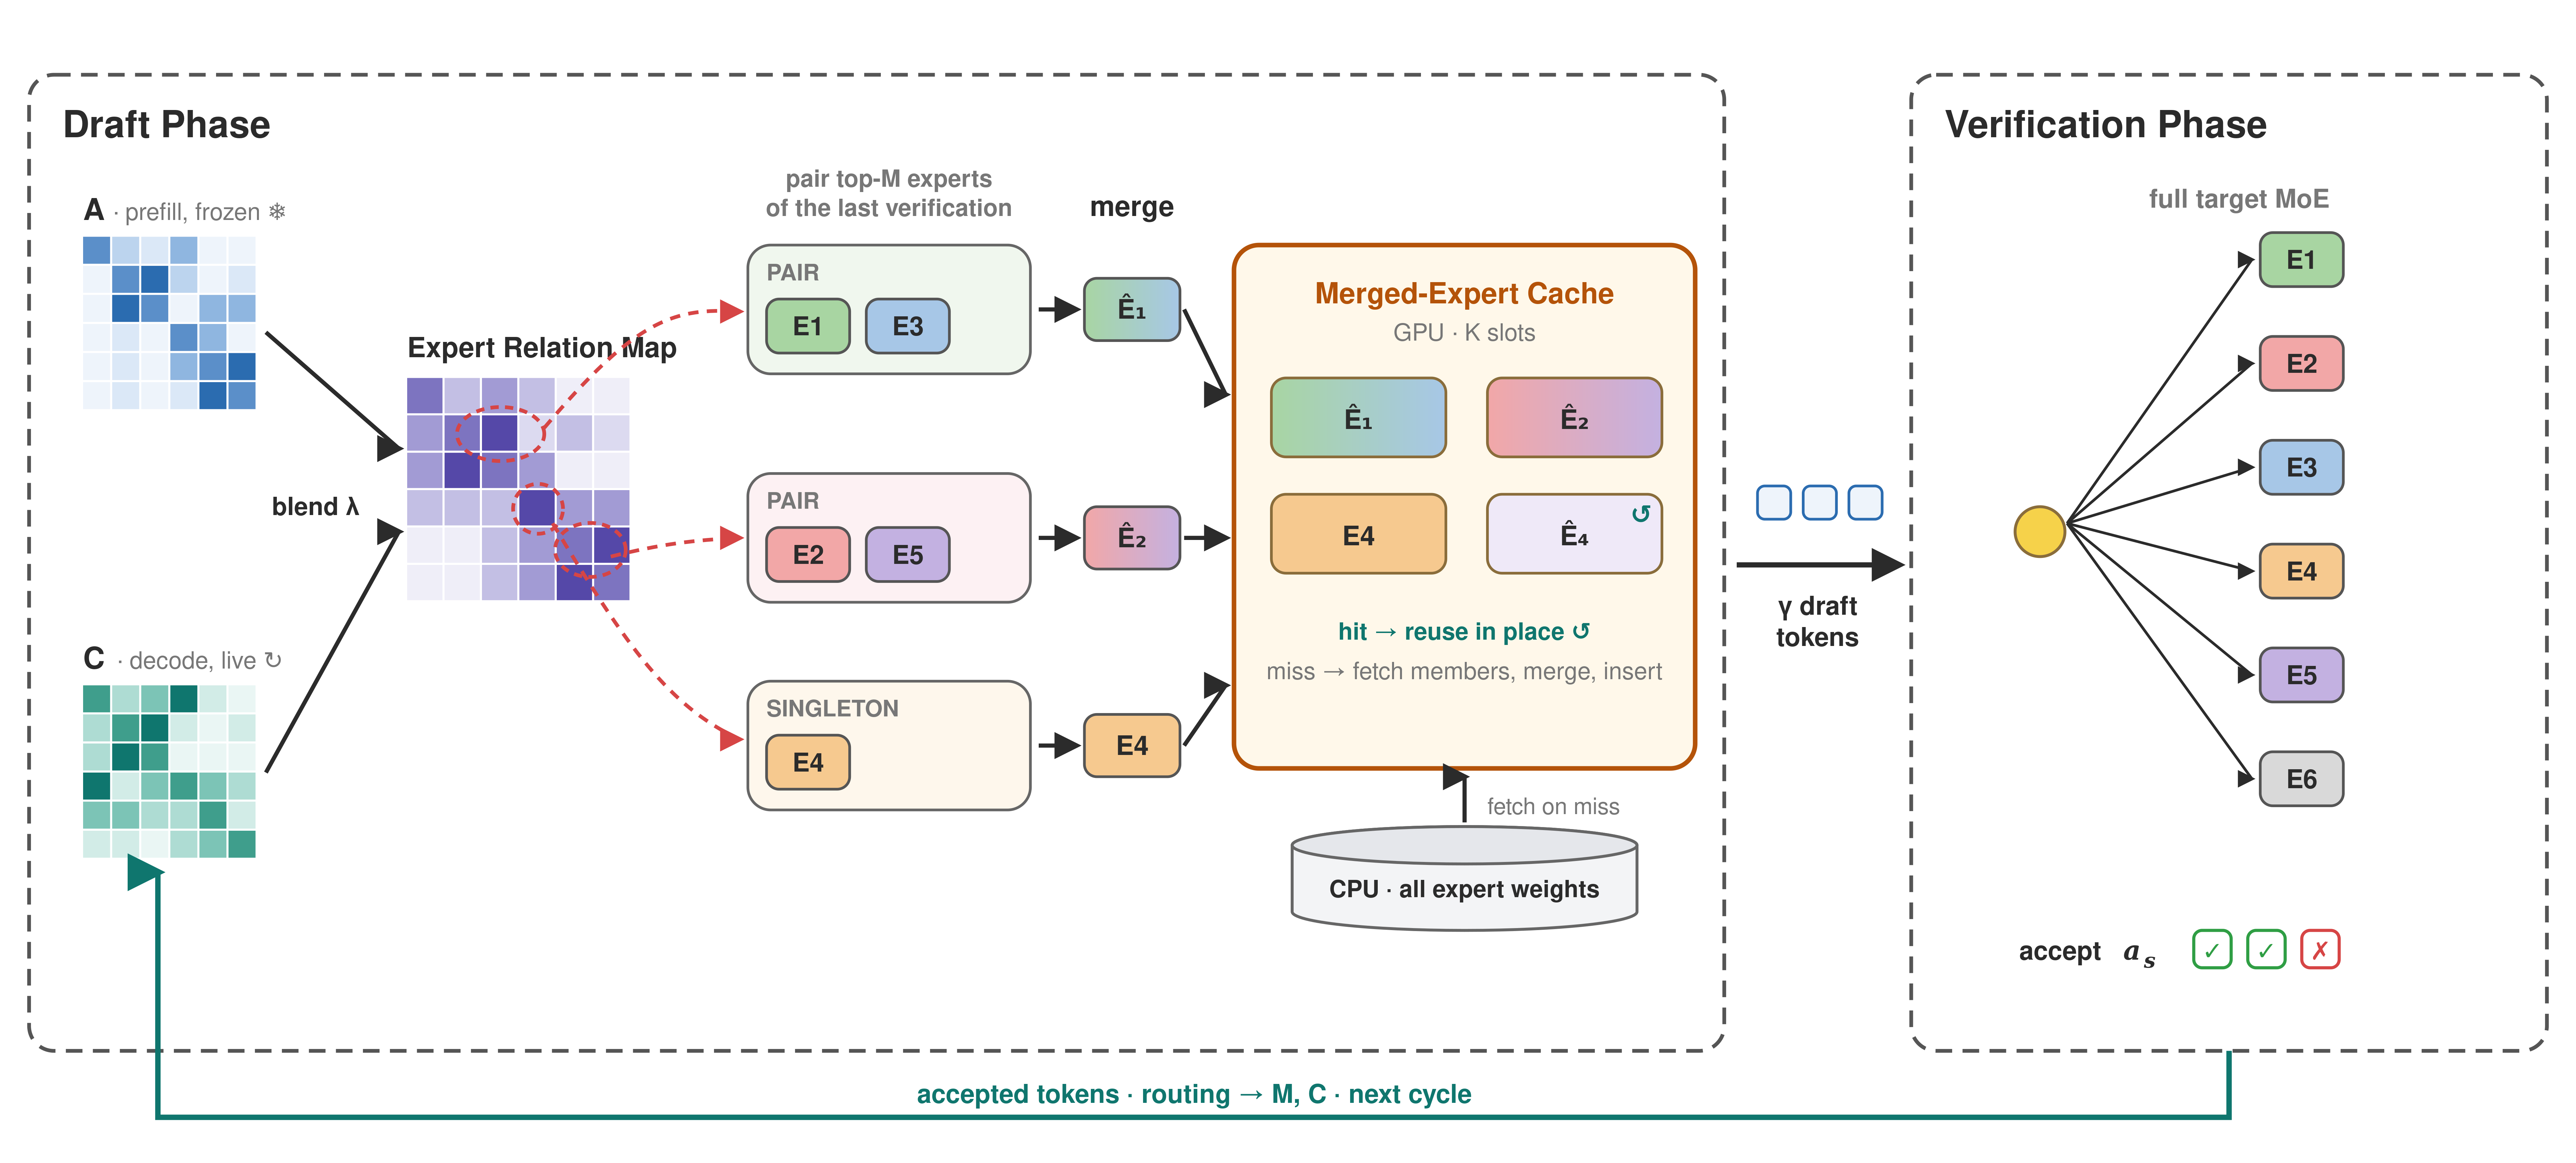
\includegraphics[width=\textwidth]{fig_method}
  \caption{Overview of MergeSpec. A single prefill pass builds the frozen
    activation-similarity map $\mathbf{A}_{\ell}$. Each draft--verify cycle
    then blends $\mathbf{A}_{\ell}$ with the live co-occurrence map
    $\mathbf{C}_{\ell}$ into the relation map $\mathbf{R}_{\ell}$, pairs the
    top-$M$ experts routed by the last verification into $K$ groups, and
    probes the GPU merged-expert cache before drafting: a hit reuses the
    resident merged expert, a miss fetches members from the CPU backing
    store and merges them in weight space. The $K$ merged experts propose
    $\gamma$ tokens, the full target MoE verifies them, and the verified
    routing updates $\mathbf{C}_{\ell}$ for the next cycle.}
  \label{fig:method}
\end{figure*}

\subsection{Expert Relation Map}

Merging preserves draft coverage only when the experts grouped together
are functionally or behaviorally related. Proposition~2 bounds the merge
error by the within-group variance, so the central question is which
experts may share a resident draft expert. MergeSpec answers this question
with an \emph{Expert Relation Map}, maintained per MoE layer $\ell$ and
per request. Figure~\ref{fig:method} shows how the map drives the full
draft--verify cycle: a prefill pass fixes the similarity structure, each
cycle blends it with the running co-occurrence signal to cluster and
merge the resident draft experts, the merged draft proposes tokens, and
the target verifier both validates them and refreshes the co-occurrence
signal for the next cycle. The map combines two signals that become
available at different stages of inference and carry different kinds of
information.

\paragraph{Activation-similarity map.}
The first signal measures functional relatedness. During the prefill
pass, the router assigns every prompt token to its top-$k$ experts, so
pairs of experts are evaluated on identical inputs. Let
$\mathcal{P}_{\ell}^{ij} = \{\, t : i \in \mathcal{T}_{\ell,t} \wedge
j \in \mathcal{T}_{\ell,t} \,\}$ denote the prefill tokens co-routed to
experts $i$ and $j$ at layer $\ell$. MergeSpec records the per-expert
outputs produced during this single pass and defines
\begin{equation}
\mathbf{A}_{\ell}[i,j] \;=\;
  -\,\frac{1}{|\mathcal{P}_{\ell}^{ij}|}
  \sum_{t \in \mathcal{P}_{\ell}^{ij}}
  \bigl\lVert E_{\ell,i}(h_{\ell,t}) - E_{\ell,j}(h_{\ell,t})
  \bigr\rVert_{2},
\label{eq:actsim}
\end{equation}
the negative mean $L_2$ distance between the two experts' outputs on
shared inputs. Larger values indicate stronger functional redundancy.
Pairs never co-routed during prefill are marked unobserved.
$\mathbf{A}_{\ell}$ is a direct empirical estimate of the quantity that
Proposition~2 requires: experts with small output distance on the current
context behave as locally aligned functions, and merging them incurs
little error. This signal has two defining properties. It is expensive to
acquire, because it requires materializing individual expert outputs
rather than only their routed sum. It is also stable, because it reflects
the functional geometry of the experts conditioned on the request context
rather than the token-by-token routing trajectory. We observe that
per-pair similarities drift little across decoding cycles. MergeSpec
therefore pays the capture cost exactly once, during prefill, and freezes
$\mathbf{A}_{\ell}$ for the remainder of the request.

\paragraph{Co-occurrence map.}
The second signal measures usage relatedness. During decoding, every
verification pass reveals the target's true routing decisions for the
tokens it validates. Let $\mathcal{V}_{s}$ denote the tokens verified up
to cycle $s$. MergeSpec accumulates
\begin{equation}
\mathbf{C}_{\ell}[i,j] \;=\;
  \bigl|\{\, t \in \mathcal{V}_{s} :
  i \in \mathcal{T}_{\ell,t} \wedge j \in \mathcal{T}_{\ell,t} \,\}\bigr|,
\label{eq:cooccur}
\end{equation}
the number of decoded tokens whose top-$k$ set contains both experts. The
diagonal $\mathbf{C}_{\ell}[i,i]$ counts each expert's activations.
$\mathbf{C}_{\ell}$ captures the temporal locality of expert usage: it
records which experts the current generation trajectory activates, and
which it activates together. Unlike $\mathbf{A}_{\ell}$, this signal is
nonstationary. As generation moves through phases of the response, the
co-activation pattern shifts, so the map must be re-estimated online.
Its acquisition cost is negligible, since the router computes
$\mathcal{T}_{\ell,t}$ regardless and the update adds no expert
computation or memory movement.

The two maps are complementary along exactly the axis that matters for
draft construction. $\mathbf{A}_{\ell}$ is reliable but static: it
identifies which experts are interchangeable, not which experts the
generation currently needs. $\mathbf{C}_{\ell}$ is adaptive but shallow:
it tracks the routing distribution as it shifts, yet it cannot certify
that co-activated experts are compatible enough to share a merged
representative. MergeSpec therefore consumes the two maps jointly, as
described next.

\subsection{Relation-Guided Cluster-and-Merge}

At each cycle, MergeSpec rebuilds the draft path from the Expert Relation
Map in two steps: it partitions the currently relevant experts into at
most $K$ groups, then merges each group into one resident draft expert.

\paragraph{Clustering.}
$\mathbf{A}_{\ell}$ is a negative distance and $\mathbf{C}_{\ell}$ is a
count, so the two maps live on incommensurable scales. Each map is first
normalised per layer by $\mathcal{N}(\cdot)$, which maps observed entries
onto $[0,1]$ by their normalised rank and places unobserved entries below
the observed range. The relation map at cycle $s$ is the convex blend
\begin{equation}
\mathbf{R}_{\ell} \;=\;
  \lambda\,\mathcal{N}\!\bigl(\mathbf{A}_{\ell}\bigr)
  \;+\;
  (1-\lambda)\,\mathcal{N}\!\bigl(\mathbf{C}_{\ell}\bigr),
\qquad \lambda \in [0,1].
\label{eq:blend}
\end{equation}
Since $\mathbf{A}_{\ell}$ is frozen after prefill while
$\mathbf{C}_{\ell}$ grows with every verified token,
Eq.~\eqref{eq:blend} re-weights a fixed functional-similarity structure
with the live temporal-locality state of the request. Experts that the
current trajectory fires together are pulled toward a shared draft
expert, but only insofar as the prefill-measured similarity certifies
that merging them is benign. The endpoints recover the pure strategies:
$\lambda{=}1$ groups by functional similarity alone, and $\lambda{=}0$
groups by co-activation alone. Clustering is then a greedy
maximum-relation matching over the candidate set $\mathcal{M}_{\ell}$,
the $M$ experts most frequently routed by the most recent verification
pass. The two statistics thus operate on complementary time windows:
$\mathbf{C}_{\ell}$ accumulates over all verified tokens and provides
long-range memory, while $\mathcal{M}_{\ell}$ is rebuilt from the latest
pass alone and keeps the draft anchored to the experts the generation is
using right now. Candidate pairs are
ranked by $\mathbf{R}_{\ell}$ in descending order and accepted greedily
under the constraint that each expert joins at most one pair, until $K$
groups remain; leftover experts stay singletons. Capping groups at two
members keeps the within-group variance small, which by Proposition~2
keeps the merge error small, while still halving the residency cost of
every paired expert.

\paragraph{Merging.}
Each group is then merged directly in weight space. Following the
construction analysed in Proposition~2, the merged draft expert
$\widehat{E}_{\ell,j}$ is realised by linearly combining the weight
matrices of its members:
\begin{equation}
\widehat{\mathbf{W}}_{\ell,j} \;=\;
  \sum_{i \in \mathcal{C}_{\ell,j}} \alpha_{\ell,j,i}\,\mathbf{W}_{\ell,i},
\qquad
\alpha_{\ell,j,i} \;=\; \frac{1}{|\mathcal{C}_{\ell,j}|},
\label{eq:weightmerge}
\end{equation}
applied independently to every projection matrix of the expert FFN (the
gate, up, and down projections in gated-MLP experts such as Qwen3).
Merging therefore requires no forward passes and no calibration data: it
is a weighted sum over weight tensors that are already resident from the
preceding verification pass. Because the group members are selected by
$\mathbf{R}_{\ell}$ to be functionally close, Proposition~2 guarantees
that this weight-space combination approximates the function-space
average of the group, which is precisely the aggregate behavior the draft
expert must reproduce.

The division of work across stages follows the cost structure of the
two maps.
Prefill processes the whole prompt in one pass, so it observes enough
co-routed tokens to populate $\mathbf{A}_{\ell}$ densely, and the capture
overhead is paid off the decoding critical path. Re-measuring similarity
at every cycle would place that overhead on the critical path in exchange
for values that barely change, so MergeSpec does not do it. Decoding
instead updates only the free routing statistics, and adapts the
partition at every cycle by re-blending the frozen similarity structure
with the current activation state. The per-cycle overhead is a sort over
at most $\binom{M}{2}$ scored pairs, which is negligible, and it keeps
the draft path aligned with where the generation is actually routing.
